\chapter{Evaluierung der Verwendbarkeit des Werkzeugs} % (fold)
\label{cha:eval_werkzeug}

Im ersten empirischen Teil der Evaluierung wurde die grundlegende Verständlichkeit und Verwendbarkeit des Werkzeug geprüft. Ziel war es hier, konzeptionelle und technische Eigenschaften bzw. Verhaltensweisen des Werkzeugs zu identifizieren, die den Modellierungsprozess behindern oder unterbrechen. Darunter fällt grundsätzlich jede Eigenschaft und jede Verhaltensweise, die die Benutzer zwingt, sich mit dem technischen System an sich zu beschäftigen und von der Erfüllung der eigentlichen Aufgabe ablenkt bzw. diese unterbricht.

Die Untersuchung wurde daneben auch genutzt, um explorativ die inhaltliche Verwendung des Systems zu untersuchen (d.h. wie es für seinen eigentlichen Verwendungszweck, die Modellierung, eingesetzt wurde) und Hypothesen abzuleiten, die in weiteren Schritten getestet werden konnten.

\section{Hypothesen} % (fold)
\label{sec:hypothesen}

In diesem Abschnitt werden die Hypothesen angeführt und begründet, die in diesem Teil der empirischen Untersuchung geprüft werden. Die hier angegebenen Hypothesen gehen auf die Eigenschaften des Werkzeugs in der Verwendung durch die Benutzer ein. Bei der Hypothesenbildung wird auf den Verwendungszweck des Werkzeugs, die Unterstützung der Bildung diagrammatischer Modelle, Rücksicht genommen -- die Modelle selbst sind jedoch nicht Gegenstand der Betrachtung, sondern werden erst im nächsten Kapitel behandelt. Nicht berücksichtigt wird außerdem die Verwendung zur Unterstützung von Articulation Work -- die Implikationen des Werkzeugs auf diese sind Gegenstand von Kapitel \ref{cha:eval_aw}.

\subsection{Konzeptionell begründete Hypothesen} % (fold)
\label{sub:konzeptionell_begründete_hypothesen}

Die folgenden Hypothesen wurden aus der Aufgabenstellung (siehe Kapitel XY) sowie den Anforderungen an das Werkzeug (siehe Kapitel XY) abgeleitet. Neben der Formulierung der Hypothese ist jeweils die Begründung aus der Konzeption des Werkzeugs angeführt.

Der grundlegende Anspruch des Werkzeugs ist es, explizite Articulation Work zu unterstützen. Wie in Teil \ref{prt:grundlagen} dieser Arbeit beschrieben, wird dies hier über die Externalisierung und Aushandlung von mentalen Modellen realisiert. Ein gängiges Mittel, um mentale Modelle zu repräsentieren, sind diagrammatische Modelle, worunter die Ergebnisse der vorgeschlagenen Methoden zur Externalisierung -- Concept Mapping und Strukturlegetechniken -- fallen. Das Werkzeug muss also die Repräsentation diagrammatischer Modelle unterstützen. 

\begin{hyp}
	\label{hyp:diagmodelle}
	Das Werkzeug ermöglicht die Repräsentation diagrammatische Modelle.
\end{hyp}

Articulation Work ist immer in einen kollaborativen Arbeitszusammenhang eingebettet. Die Kollaboration findet dabei nicht nur im produktiven Teil der Arbeit statt, sondern hat immer auch Auswirkungen auf die Articulation Work. Jede Unterstützung von Articulation Work muss damit auch in kollaborativen Szenarien einsetzbar sein. Dies gilt auch für das hier vorgestellte Werkzeug, das die kollaborative Bearbeitung einer Aufgaben (hier: der Externalisierung und Abstimmung mentaler Modelle) ermöglichen muss. 

\begin{hyp}
	\label{hyp:kollaborativ}
	Das Werkzeug ermöglicht kollaboratives Arbeiten an einer Aufgabe.
\end{hyp}

Die Aspekte von Arbeit, die im Rahmen von Articulation Work abzustimmen sind, sind unterschiedlicher Natur. Naheliegend ist eine Abstimmung der Abläufe und Schnittstellen zwischen Personen, aber auch nicht-prozedurale Information wie das Verständnis der Struktur und Elemente eines Arbeitszusammenhangs kann Gegenstand von Articulation Work sein. Gleiches gilt für die im Rahmen der Articulation Work abzustimmenden mentalen Modelle -- diese bilden die Basis für Handlungsentscheidungen, umfassen aber im Allgemeinen (in Abgrenzung zu Schemata) nicht nur handlungsleitende Information sondern auch Kontextinformation, die die Bewertung der wahrgenommenen Situation ermöglicht. Demensprechend muss ein Werkzeug zu Unterstützung von expliziter Articulation Work und damit der Externalisierung von mentalen Modellen die Verwendung in unterschiedlichen Kontexten, d.h. für unterschiedliche zu externalisierenden Informationsstrukturen, die in mentalen Modellen abgebildet sind, ermöglichen.

\begin{hyp}
	\label{hyp:kontexte}
	Das Werkzeug ist gleichwertig für Modellierungsaufgaben in unterschiedlichen Kontexten einsetzbar.
\end{hyp}

Die ersten drei hier formulierten Hypothesen sind unmittelbar aus der globalen Zielsetzung abgeleitet und bilden die grundlegenden Anforderungen an das Werkzeug bei der Unterstützung von Articulation Work ab. Die nun folgenden Hypothesen sind konzeptionell nicht mehr direkt auf die globale Zielsetzung ausgerichtet sondern stellen auf Funktionalität des Werkzeugs ab, die den Modellbildungsprozess unterstützen soll. 

Die erste dieser Hypothesen bildet eine wesentliche Funktionalität des Werkzeugs, nämlich die Möglichkeit durch die Entstehungsgeschichte des erstellten Modells zu navigieren, ab. In der dieser Funktionalität zugrundeliegenden Literatur (\citep{Shipman00}, \citep{Klemmer02}) wird diese als wesentlich bezeichnet, wenn Externalisierungsprozesse unterbrochen werden, kollaborativ durchgeführt werden oder Dritten die Möglichkeit gegeben werden soll, die Entstehung des Modells nachzuvollziehen. Allen drei Aspekten liegt die Annahme zugrunde, dass in der Historie des Externalisierungsprozesses die dem Ergebnis zugrundeliegenden Ideen und Annahmen zu erkennen sind. Im Kontext dieser Arbeit bedeutet dies, dass aus der Nachverfolgung der Historie des externalisierten Modells die diesem zugrundeliegenden mentalen Modelle verständlich und nachvollziehbar werden. 

\begin{hyp}
	\label{hyp:historie}
	Die Reflexion des Modellierungsverlaufs ermöglicht das Verständnis der dem Modell zugrundeliegenden mentalen Modelle.
\end{hyp}

Auf Basis der Möglichkeit zur Navigation durch die Entstehungsgeschichte des Modells besteht auch die Möglichkeit, vergangene Modellzustände wiederherzustellen. Das Werkzeug unterstützt dabei die Benutzer durch die Ausgabe von schrittweisen Anweisungen, die den aktuellen Modellzustand in den wiederherzustellenden Zustand überführen. Allgemein bietet diese Funktionalität die Möglichkeit, erkannte Fehler im Modell zu korrigieren, ohne dabei bereits repräsentierte Information zu verlieren. Im kollaborativen Einsatz ermöglicht diese Funktionalität, alternative, individuelle Sichten auf den abzustimmenden Sachverhalt zu repräsentieren und dabei die Möglichkeit bieten, einen für alle Beteiligten akzeptablen Ausgangspunkt wiederherzustellen

\begin{hyp}
	\label{hyp:wiederherstellung}
	Die Möglichkeit der Wiederherstellung vergangener Modellzustände fördert die Bereitschaft alternative Repräsentationen auszuprobieren.
\end{hyp}

Die letzten beiden Hypothesen dieses Abschnitts sind ausschließlich auf die Verwendung des Werkzeugs an sich ausgerichtet und stehen nicht im Kontext von Articulation Work oder der Unterstützung der Externalisierung mentaler Modelle. Hypothese \ref{hyp:behinderung} steht für den in der Zielsetzung formulierten Anspruch, dass das Werkzeug in den Hintergrund treten muss und die Beschäftigung mit der eigentlichen Aufgabe nicht behindern darf. Dabei wird hier nicht auf den konkreten Anwendungsfall -- die Erstellung von Modellen -- eingegangen sondern lediglich die allgemeine Funktionsfähigkeit und Bedienbarkeit des Werkzeugs betrachtet. Ersteres ist Gegenstand der Evaluierung der erstellten Modelle, die in Kapitel \ref{cha:eval_modell} beschrieben werden.

\begin{hyp}
	\label{hyp:behinderung}
	Das Werkzeug behindert die Modellbildung nicht.
\end{hyp}

Hypothese \ref{hyp:gewöhnung} geht davon aus, dass bei wiederholten Verwendung des Werkzeugs Lern- und Gewöhnungseffekte auftreten, die die Verwendung erleichtern, beschleunigen und zu weniger Fehlbedienung führen. Dies ist ein Effekt, der bei jedem Werkzeug zu erwarten ist, dessen zugrundeliegenden Konzepte den Benutzern bewusst sind. Von dieser Voraussetzung kann durch die inhaltliche Einführung der Benutzer in die das Werkzeug prägenden und motivierenden Ideen ausgegangen werden. Damit wäre zu erwarten, dass das Werkzeug bei wiederholtem Einsatz in den späteren Anwendungen effizienter (im Sinne von schneller und Fehlbedienungen vermeidend) verwendet wird.

\begin{hyp}
	\label{hyp:gewöhnung}
	Wiederholte Verwendung des Werkzeugs führt zu schnellerer Modellbildung und weniger Fehlbedienungen.
\end{hyp}

% subsection konzeptionell_begründete_hypothesen (end)

\subsection{Explorativ gebildete Hypothesen} % (fold)
\label{sub:explorativ_gebildete_hypothesen}

Neben den aus der Aufgabenstellung abgeleiteten Hypothesen wurden einige Hypothesen auch während der Durchführung der einzelnen Evaluierungs-Blöcke gebildet. Diese Hypothesen sind spezifischer auf einzelne Aspekte des Werkzeugs abgestellt und decken beobachtete Auffälligkeiten und Missverständnisse in der Verwendung des Werkzeugs ab. 

Die erste in diesem Zusammenhang beobachtete Auffälligkeit betrifft die Herstellung von Verbindern zwischen einzelnen Modellelementen. Wie in Abschnitt \ref{sub:verbinden_von_modellelementen} beschrieben, existieren zwei Möglichkeiten, diese Funktion auszuführen. Einerseits können die beiden Modellelemente, die verbunden werden sollen, mit Markierungs-Tokens ausgewählt werden, worauf hin eine Verbindung hergestellt werden. Andererseits können Verbinder auch durch das Zusammenführen der zu verbindenden Blöcke (bis sich deren Breitseiten berühren) hergestellt werden. In der ersten Implementierung des Werkzeugs, die im Evaluierungs-Block 1 und im ersten Teil des zweiten Blocks verwendet wurde, war lediglich die erste Variante verfügbar. Die Möglichkeit zur Herstellung von Verbindern wurde in den in diesen Blöcken durchgeführten Anwendungen kaum eingesetzt. Dies führte einerseits zur Bildung der Hypothese \ref{hyp:keineverbinder} (siehe Abschnitt \ref{sub:m_explorativ_gebildete_hypothesen}), andererseits wurde bei ersten Auswertungen der Beobachtungen der im Verhältnis zum übrigen Modellierungs-Prozess hohe Zeit-Aufwand bei der Herstellung von Verbindern offensichtlich. Dieser Aufwand ist den Maßnahmen zur Stabilisierung der Erkennungsleistung des Werkzeugs geschuldet und kann mit den eingesetzten Interaktionsablauf nicht reduziert werden. Aufgrund einer Anregung eines Untersuchungsteilnehmers wurde deshalb die oben beschriebene zusätzliche Möglichkeit zur Herstellung von Verbindungen implementiert. Zu untersuchen ist nun, ob diese Maßnahme die Nutzung von Verbindern bei der Modellbildung tatsächlich erhöht.

\begin{hyp}
	\label{hyp:verbinder}
	Die Einführung der alternativen Möglichkeit zur Verbindungsherstellung erhöht die Nutzung von Verbindern bei der Modellerstellung.
\end{hyp}

Die zweite hier aufgestellte Hypothese betrifft eine Auffälligkeit bei der Verwendung des Löschtokens. Das Löschtoken wird verwendet, um das Werkzeug in einen Modus zu versetzen, in dem Verbinder gelöscht werden können. Schon die konzeptionelle Einordnung des Werkzeugs in Kapitel \ref{cha:konzeptionelle_evaluierung} zeigte Potential für Missverständnisse in der Verwendung dieses Tokens (siehe z.B. die Abschnitte \ref{sec:spezifikation_des_tac_schemas_nach_shaer_et_al_} und \ref{sec:einordnung_in_die_taxonomie_von_fishkin}). Zusammengefasst liegt die aus der Theorie ableitbare Problematik darin, dass durch die äußere Form des Tokens -- einem Radiergummi -- eine Metapher für dessen Verwendung („ausradieren“ von Elementen) suggeriert wird, die in dieser Form im Werkzeug nicht umgesetzt ist, da das Token lediglich als Schalter fungiert. Erste Beobachtungen deuteten darauf hin, dass die Verwendung des Löschtoken tatsächlich unverständlich oder missverständlich zu sein scheint. Die zugehörige Hypothese ist positiv formuliert, zu erwarten wäre demnach, dass sie verworfen werden muss.

\begin{hyp}
	\label{hyp:radierer}
	Das Löschtoken ermöglicht intuitives Löschen von Modellelementen.
\end{hyp}

% subsection explorativ_gebildete_hypothesen (end)
% section hypothesen (end)

\section{Untersuchungsdesign und Durchführung} % (fold)
\label{sec:untersuchungsdesign}

In diesem Abschnitt wird auf Basis der eben formulierten Hypothesen ein Untersuchungsdesign abgeleitet und die Durchführung der Untersuchung beschrieben. Im ersten Schritt werden die Hypothesen hinsichtlich der Möglichkeiten ihrer Beurteilung betrachtet und dabei die zu erhebenden Variablen identifiziert. Im nächsten Schritt folgt die Operationalisierung, in der die konkrete Messung bzw. Beurteilung der einzelnen Variablen festgelegt wird. Aus dieser Operationalisierung können die durchzuführenden Untersuchungen abgeleitet werden. An dieser Stelle erfolgt auch die Einordnung in die in Kapitel \ref{cha:eval_ueberblick} beschriebenen Evaluierungsblöcke. Im letzten Teil dieses Abschnitts wird die eigentliche Durchführung beschrieben, wobei im Speziellen auf deskriptive Parameter der Untersuchung eingegangen wird, die im Kontext der Werkzeugverwendung von Interesse sind, aber nicht oder nur als Teil der Berechnungsgrundlage in die Auswertung der Hypothesen eingehen.

\subsection{Operationalisierung} % (fold)
\label{sub:operationalisierung}

In diesem Abschnitt wird für jede Hypothese identifiziert, welche Variablen bei ihrer Beurteilung berücksichtigt werden müssen. Für jeder der Variablen wird in der Folge die konkrete Mess- und Auswertungsmethode festgelegt (auf Basis der in Abschnitt \ref{sec:eingesetzte_werkzeuge_und_verfahren} beschriebenen Verfahren).  

\subsubsection{Repräsentation} % (fold)
\label{ssub:repräsentation}

% subsubsection repräsentation (end)

\subsubsection{Kollaboratives Arbeiten} % (fold)
\label{ssub:kollaboratives_arbeiten}

Abhängige Variable: Zeitverteilung der Beteiligung der Benutzer (quant), gleichzeitige Manipulation (qual)

% subsubsection kollaboratives_arbeiten (end)

\subsubsection{Einsetzbarkeit in unterschiedlichen Kontexten} % (fold)
\label{ssub:einsetzbarkeit_in_unterschiedlichen_kontexten}

Abhängige Variable: Modellgröße in Abhängigkeit der Modellierungdauer (quant), Aussagen der Benutzer (qual)
Idee: Wenn die Modellgröße mit der Modellierungsdauer positiv korreliert, ist der Zeitanteil, der zur Beschäftigung mit dem Werkzeug notwendig ist, immer gleich groß, d.h. verändert sich nicht zwischen den Anwendungen. 

Unabh. Var.: Tisch, Modellierungsaufgabe

% subsubsection einsetzbarkeit_in_unterschiedlichen_kontexten (end)

\subsubsection{Nicht-Behinderung} % (fold)
\label{ssub:nicht_behinderung}

Abhängige Variable: Notwendige Korrekturen von Fehlfunktionen des Tisches, Systemabstürze (quant.), Empfinden der Benutzer (qual).

% subsubsection nicht_behinderung (end)

\subsubsection{Gewöhnnung an das Werkzeug} % (fold)
\label{ssub:gewöhnnung_an_das_werkzeug}

Abhängige Variable: Fehlbedienungen in Abhängigkeit des Durchgangs, Modellierungsdauer in Abhängigkeit des Durchgangs

Störvariablen: Modellgröße (Korrelation mit Dauer), Veränderte Funktionalität des Werkzeugs

% subsubsection gewöhnnung_an_das_werkzeug (end)

\subsubsection{Herstellung von Verbindern} % (fold)
\label{ssub:herstellung_von_verbindern}

Unabh. Variable: Modellierungs-Tisch
Abhängige Variable: Connectedness (quant)
Störvariable: Modellierungsaufgabe

Störvariable ausgeschaltet, indem die Signifikanz der Änderung der Connectedness zwischen zwei Blöcken mit gleicher Grundgesamtheit und gleicher Aufgabenstellung gemessen wird.

% subsubsection herstellung_von_verbindern (end)

\subsubsection{Löschtoken} % (fold)
\label{ssub:löschtoken}

Abhängige Variablen: Anzahl der Fehlbedienungen im Verh. zu allen Anwendungen (quant), Art des Missverständnisses (qual) 

% subsubsection löschtoken (end)

% subsection operationalisierung (end)

\subsection{Datenbasis} % (fold)
\label{sub:datenbasis}

Als Grundlage der Überprüfung der Hypothesen werden hier die Evaluierungs-Blöcke 1 bis 5 verwendet. Dabei wurden für die quantitativ zu prüfenden Variablen die Blöcke 2 und 3 herangezogen. In die qualitative Auswertung der Ergebnisse wurden hingegen alle Blöcke (1-5) mit einbezogen.

% subsection datenbasis (end)

\subsection{Durchführung} % (fold)
\label{sub:durchführung}

In diesem Abschnitt werden die für diesen Evaluierungs-Teil relevanten deskriptiven Parameter der berücksichtigten Anwendungs-Blöcke angeführt.

\subsubsection{Stichprobe} % (fold)

\begin{tabular}{| p{2cm} || p{2,5cm} | p{2,5cm} | p{2,5cm} || p{2cm} |}
  \hline
   & Aushandlung (1. Durchgang) & Aushandlung (2. Durchgang) & Concept Mapping & Gesamt \\ \hline
   $n_{Anwendungen}$ & 9 & 9 & 17 & 35 \\ 
   $n_{Teilnehmer}$ & 19 & 18 & 47 & 84 \\ \hline
\end{tabular} 

\subsubsection{Dauer der Werkzeugverwendung} % (fold)

Die Dauer der Werkzeug-Verwendung wurde den Blöcken 2 („Aushandlung“) und 3 („Concept Mapping“) erhoben. Die Bearbeitungszeit ist wie folgt verteilt (siehe auch Abbildung \ref{fig:img_Evaluierung_usageTimeOverview}\footnote{In allen Boxplots gilt folgende Notation: 
\begin{itemize}
	\item breite horizontale Linie: Bereich zwischen 25\%- und 75\%-Quantil
	\item breite vertikale Linie: Median
	\item linke schmale Linie: Bereich zwischen 2,5\%- und 25\%-Quantil
	\item rechte schmale Linie: Bereich zwischen 75\%- und 97,5\%-Quantil
	\item Kreuze: Ausreißer (außerhalb 2,5\%- und 97,5\%-Quantil)
\end{itemize}
}):

\begin{tabular}{| p{1cm} || p{3cm} | p{3cm} | p{3cm} |}
  \hline
   & Aushandlung (1. Durchgang) & Aushandlung (2. Durchgang) & Concept Mapping \\ \hline
   $t_{min}$ & 11m 54s & 2m 5s & 14m 1s \\ 
   $\overline{t}$ & 20m 53s & 9m 49s & 32m 32s \\ 
   $s(t)$ & 4m 18s & 5m 20s & 10m 7s \\
   $t_{max}$ & 27m 30s & 19m 29s & 45m 0s \\ \hline
\end{tabular} 

\begin{figure}[htbp]
	\centering
		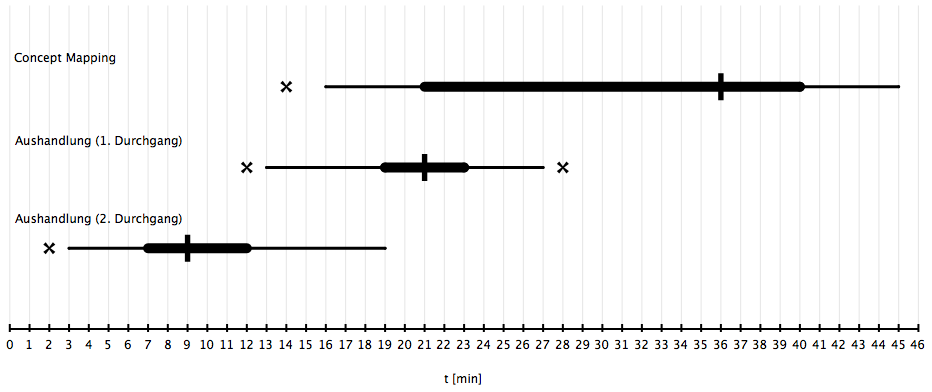
\includegraphics[width=15cm]{img/Evaluierung/usageTimeOverview.png}
	\caption{Dauer der Werkzeugverwendung -- Überblick}
	\label{fig:img_Evaluierung_usageTimeOverview}
\end{figure}

Die erhobene Dauer der Werkzeug-Verwendung teilt sich ein einen Anteil, an dem tatsächlich mit dem Werkzeug interagiert wird und einen Anteil, der anderen Tätigkeiten (wie inhaltlicher Diskussion, Bedeutungsaushandlung, \ldots) gewidmet ist. Diese beiden Anteile sind in den einzelnen Blöcken wie folgt verteilt (siehe auch die Abbildungen \ref{fig:img_Evaluierung_usageTimeConceptMapping} und \ref{fig:img_Evaluierung_usageTimeNegotiation}):

\begin{figure}[htbp]
	\centering
		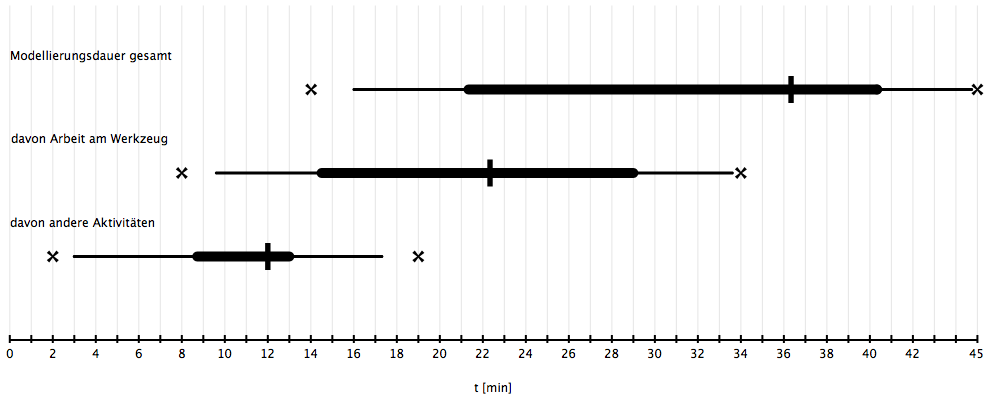
\includegraphics[width=15cm]{img/Evaluierung/usageTimeConceptMapping.png}
	\caption{Dauer der Werkzeugverwendung -- Concept Mapping}
	\label{fig:img_Evaluierung_usageTimeConceptMapping}
\end{figure}

\begin{figure}[htbp]
	\centering
		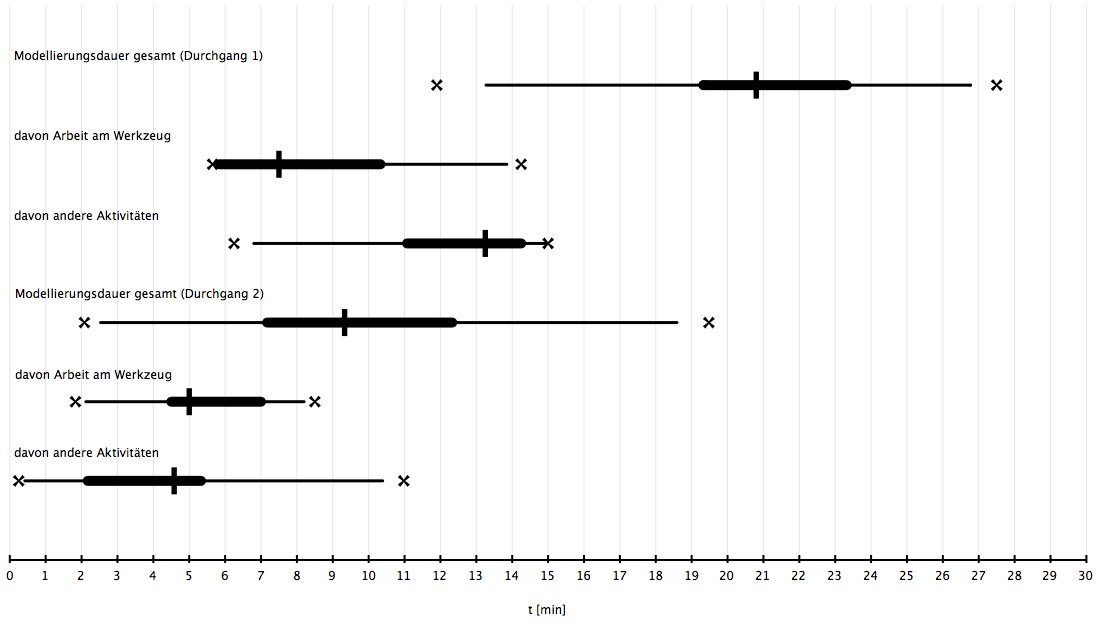
\includegraphics[width=15cm]{img/Evaluierung/usageTimeNegotiation.png}
	\caption{Dauer der Werkzeugverwendung -- Aushandlung}
	\label{fig:img_Evaluierung_usageTimeNegotiation}
\end{figure}

% subsection durchführung (end)
% section untersuchungsdesign (end)

\section{Ergebnisse} % (fold)
\label{sec:ergebnisse}

\subsection{Repräsentation diagrammatischer Modelle} % (fold)
\label{sub:repräsentation_diagrammatischer_modelle}

\subsubsection{Auswertung} % (fold)

\subsection{Diskussion} % (fold)

% subsection repräsentation_diagrammatischer_modelle (end)

\subsection{Kollaboratives Arbeiten} % (fold)
\label{sub:kollaboratives_arbeiten}

\subsubsection{Auswertung} % (fold)

\subsection{Diskussion} % (fold)

% subsection kollaboratives_arbeiten (end)

\subsection{Erstellen von Verbindungen} % (fold)
\label{sub:erstellen_von_verbindungen}

\subsubsection{Auswertung} % (fold)

\subsection{Diskussion} % (fold)

% subsection erstellen_von_verbindungen (end)

\subsection{Verwendung des Löschtokens} % (fold)
\label{sub:verwendung_des_löschtokens}

In diesem Abschnitt werden die Ergebnisse der Überprüfung der Hypothese \ref{hyp:radierer} („Das Löschtoken ermöglicht intuitives Löschen von Modellelementen.“) vorgestellt.

\subsubsection{Auswertung} % (fold)

\begin{transkript}
	\emph{Die Teilnehmer möchten einen Block umbenennen.}\\
	\textbf{A:} Wie haben wir jetzt gesagt \emph{(markiert den roten Baustein)} keine Modellierungsvorgabe \emph{(gibt Bezeichnung ein)}\\
	\emph{System übernimmt die neue Beschriftung für den Baustein nicht.}\\
	\textbf{A:} Wo wurde das hingeschrieben? \emph{(Pause)} Radiergummi? Glaubst du kann man das wegradieren?\\
	\textbf{B:} Probiere es aus.\\
	\textbf{\emph{A legt Radiergummi zum Block mit der Absicht die Beschriftung zu löschen}}\\
	\textbf{B:} Nein! Du löscht alles. Hör auf! \\
	\textbf{A:} Ok wie war das zuerst? Lassen wir das mal weg. \emph{(legt Baustein zur Seite)}\\
	\emph{A legt den Block zur Seite.} 
\end{transkript}

Ein ähnliches Missverständnis zeigt sich auch in folgender Situation:

\begin{transkript}
	\emph{TLN A und B stellen jeweils ihren Marker zu den Blöcken, die verbunden werden sollen. Dabei wird eine gerichtete Verbindung erstellt.}\\
	\textbf{C:} Jetzt haben wir aber einen Pfeil gebastelt.\\
	\textbf{B:} Ja stimmt. Interessant.\\
	\textbf{A:} Wie war das mit dem Radiergummi. \emph{(nimmt Radiergummi und legt ihn auf die Verbindung)}\\
	\textbf{B:} Nein\\
	\textbf{C:} Nein, mit dem Glas! Du löscht alles!\\
	\textbf{A:} Nein nur die Verbindung. \textbf{\emph{(Macht Radierbewegungen auf der Verbindung)}}\\
	\textbf{C:} Ich glaube dass wir das Glas nehmen müssen.\\
	\emph{A schiebt die Blöcke zwischen denen die Verbindung gelöscht werden soll zusammen.}\\
	\textbf{A:} Da es funktioniert. \emph{(schiebt die Blöcke weiter auseinander und bemerkt dass die Verbindung nicht gelöscht wurde)} Nein.\\
	\textbf{B:} Ich glaube der Radiergummi vernichtet alles.\\
	\textbf{A:} Nein der Radiergummi vernichtet nur Verbindungen. Nur welche? \emph{(schiebt beide Blöcke wieder zusammen – nimmt Radiergummi weg und schiebt Blöcke in die Ausgangsposition)}
\end{transkript}

\begin{transkript}
	\emph{Es wird eine falsche Beschriftung eingefügt. Die Teilnehmer wollen diese löschen, verwenden den Radiergummi allerdings falsch.}\\
	\textbf{B:} Aber irgendwie steht jetzt Ereignisse nicht bei dem Ding \emph{(zeigt auf gelben Block)} sondern dort \emph{(zeigt auf beschriftete Verbindung)}.\\
	\emph{A verrückt den gelben Block ein wenig.}\\
	\textbf{B:} Normal ist das nicht oder?\\
	\textbf{C:} Nein.\\
	\emph{A nimmt den Radiergummi.}\\
	\textbf{A:} Ich glaube das. \emph{(setzt den Radiergummi auf die Arbeitsfläche)}\\
	\textbf{C:} Aber nicht alles!\\
	\emph{A nimmt Radiergummi wieder weg. System erstellt eine Verbindung zwischen zwei roten Blöcken. Teilnehmer lachen. \textbf{A legt Radiergummi auf die erstellte Verbindung, und nimmt ihn wieder weg.} A nimmt die beiden verbundenen Blöcke und verschiebt sie.}\\
	\textbf{A:} Vielleicht so. \emph{(führt die Blöcke zusammen)}
\end{transkript}

\begin{transkript}
	\emph{In der Szene erstellt das System einen ungewollten Verbinder, die Teilnehmer versuchen auf verschiedene Arten den Verbinder zu löschen.}\\
	\textbf{B:} Und wie kann ich die Verbindungen löschen?\\
	\textbf{B:} Warte einmal, da gibt es irgendwo das mit dem Radiergummi.\\
	\textbf{A:} murmelt zustimmend \\
	\emph{\textbf{B nimmt den Radiergummi und platziert ihn direkt auf dem Verbinder}}\\
	\emph{Das System färbt den Tisch rot}\\
	\textbf{A:} Nein, warte. Da löscht du Alles!\\
	\emph{\textbf{B verschiebt den Radiergummi auf dem Tisch, hebt ihn an und platziert ihn direkt auf einem Block.}}\\
	\emph{Sobald der Radiergummi von der Oberfläche auf den Block gelegt wurde, entfernt das System die rote Färbung.}\\
	\textbf{A:} Ich glaube da löscht du Alles.\\
	\emph{B legt den Radiergummi an mehreren Stellen trotz der Warnung von TN A auf die Oberfläche}\\
	\textbf{B:} Nein, es will eh nicht.\\
\end{transkript}

\begin{transkript}
	\emph{C versucht die Benennung eines Verbinders mittels Radiergummi zu entfernen.}\\
	\textbf{B:} Aber irgendwie steht jetzt Ereignisse nicht bei dem Ding \emph{(deutet auf einen Block)} sondern dort \emph{(deutet auf einen Verbinder)}. Das wollen wir nicht oder?\\
	\textbf{A:} Nein.\\
	\textbf{C:} Ich glaube das. \emph{\textbf{(nimmt den Radiergummi und legt ihn auf den Verbinder den die Teilnehmer entfernen wollen.)}}\\
	\textbf{A:} Aber nicht alles.\\
	\emph{C entfernt den Radiergummi wieder von der Modellierungsoberfläche. In diesem Moment erstellt das System automatisch einen neuen Verbinder. C versucht den neuen Verbinder mittels Radiergummi zu entfernen.}\\
	\textbf{A:} Oh Gott.\\
	\textbf{C:} Vielleicht so \emph{(schiebt die beiden betroffenen Blöcke zusammen)}, nein.\\
	\textbf{B:} Nein.\\
	\textbf{A:} Oh Gott oh Gott oh Gott.\\
	\textbf{B:} Gehen wir einen Prozessschritt zurück.\\
	\textbf{C:} Genau.\\
\end{transkript}

\begin{transkript}
	\emph{Teilnehmer versuchen mit dem Radiergummi und nur einem anderen Marker einen Verbinder zu entfernen.}\\
	\textbf{B:} Können wir die nicht so auch einfach löschen?\\
	\textbf{C:} Ja mit dem Radiergummi.\\
	\textbf{B:} Muss ich den jetzt zuerst so \emph{(Hält den Radiergummi zur Kamera)} hinhalten?\\
	\textbf{A:} Nein, ich glaube, \textbf{den musst du einfach da \emph{(zeigt auf den Verbinder)} drauf legen.}\\
	\emph{B legt den Radiergummi auf den vom System automatisch erstellten Verbinder.}\\
	\textbf{A:} Und jetzt muss man \emph{(legt ein Markierungtoken auf den Verbinder)} Nein.\\
	\emph{Der Verbinder lässt sich auf diese Art nicht löschen und die Teilnehmer entscheiden sich den Fehler mittels der Wiederherstellungsfunktion zu beseitigen.}
\end{transkript}

\subsection{Diskussion} % (fold)

% subsection verwendung_des_löschtokens (end)
% section ergebnisse (end)

% chapter eval_tui (end) 